\documentclass{article}
\usepackage{fontspec}
\usepackage{polyglossia}
\setdefaultlanguage{french}
\usepackage[a4paper,margin=1cm]{geometry}

\usepackage{amsmath}
\usepackage{amssymb}
\usepackage{array}
\usepackage{auto-pst-pdf}
\usepackage{booktabs}
\usepackage{cite}
\usepackage{graphicx}
\usepackage{lmodern}
\usepackage{marvosym}
\usepackage{mathrsfs}
\usepackage{minted}
\usepackage{multicol}
\usepackage{multirow}
\usepackage{paralist}
\usepackage{schemabloc}
\usepackage{siunitx}
\usepackage{soul}
\usepackage{tikz}
\usepackage[european,cuteinductors,siunitx]{circuitikz}
\usepackage{url,hyperref}
\usepackage{verbatim}
\usepackage{xunicode,xltxtra}

\title{
\includegraphics{../../../images/inp-enseeiht} \\ ~ \\ ~ \\ ~ \\ ~ \\ Modélisation Comportementale}
\author{François Pierron \& Guilhem Saurel}
\date{\oldstylenums{\today}}

\begin{document}

\begin{titlepage}
    \setcounter{page}{0}
    \maketitle
    \vfill
    \tableofcontents
    \thispagestyle{empty}
\end{titlepage}

\section{PLL}

\subsection{Principe}
La boucle à Verrouillage de Phase (ou Phase-Locked Loop) est un dispositif permetant à un Oscillateur Contrôlé en Tension (ou Voltage Controlled Oscillator) de se verrouiller sur un signal entrant.

~

Pour obtenir notre PLL, nous avons donc pris un module ELAPLACE afin de modéliser un filtre passe-bas, connecté à un VCO (composant VCO\_sqr), dont la sortie est rebouclée sur l’entrée via un multiplieur (composant MULT).

Pour adapter les différents niveaux fournis par les composants, il a suffit d’utiliser des EVALUE et de leur donner des fonctions affines pour obtenir ce dont nous avions besoin.

~

Suivant les applications, la sortie utile de cette PLL peut se situer soit sur l’entrée du VCO (dans le cas d’une démodulation, par exemple), soit sur sa sortie (par exemple dans le cas de notre multiplieur de fréquence).

\subsection{Schématique}

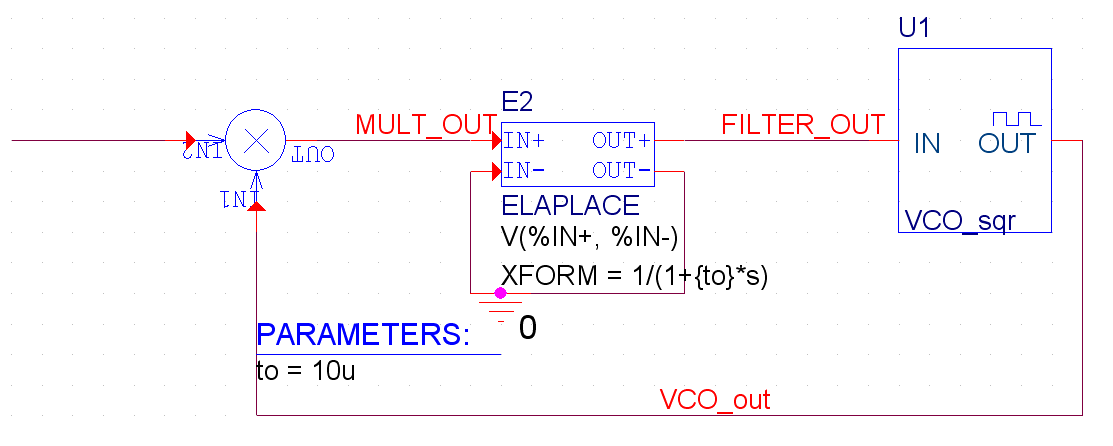
\includegraphics[width=\linewidth]{pll_sch.png}

\subsection{Résultats}

Analyser les performances d’une PLL seule n’est pas facile ; nous avons donc décidé de l’utiliser dans deux applications, une utilisant chaque sortie, et de vérifier le bon fonctionnement de ces applications.

\section{MODEM}

\subsection{Principe}

Un MODEM est composé d’une première partie modulant en fréquence un signal quelconque (mais dons la fréquence reste tout de même très inférieure à celle du signal porteur), et d’une seconde partie tentant de démoduler ce signal.

Pour la partie modulation, un VCO suffit ; et pour la démodulation nous utilisons notre PLL en regardant la sortie du filtre passe bas.

\subsection{Schématique}

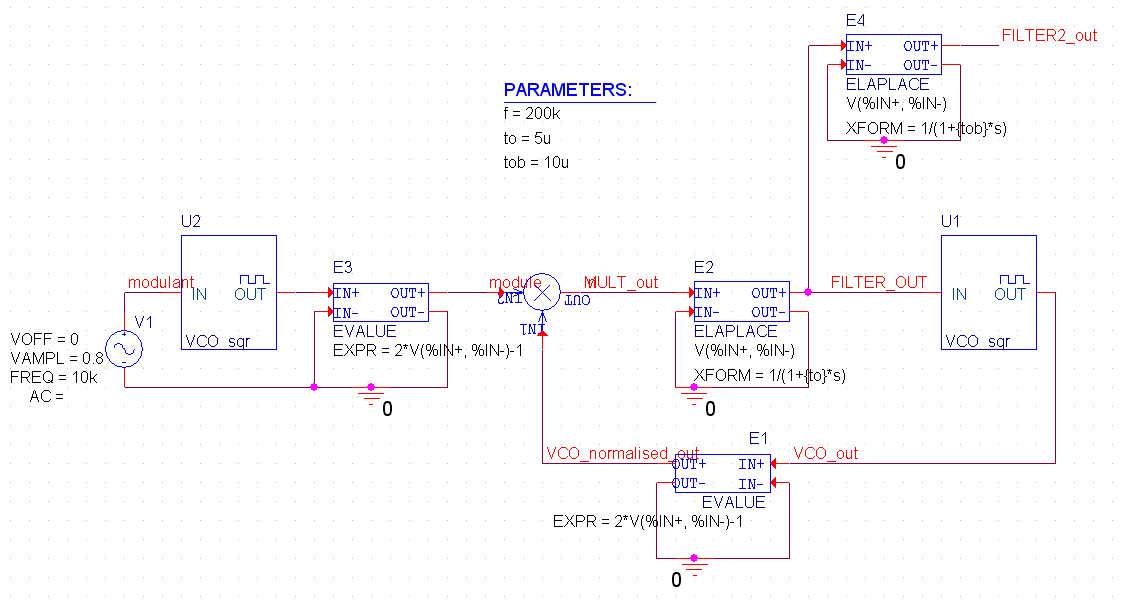
\includegraphics[width=\linewidth]{modem_sch.png}

\subsection{Résultats}

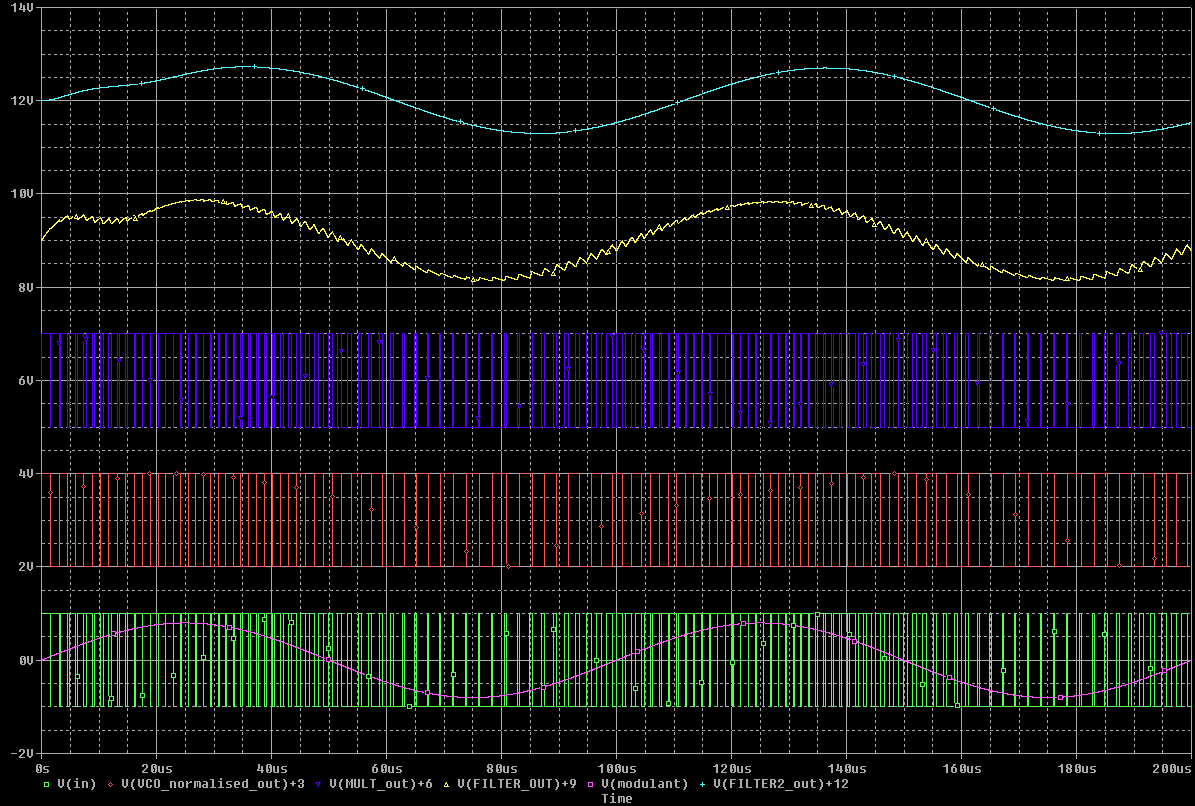
\includegraphics[width=\linewidth]{modem_sim.png}

\section{Multiplieur de fréquence}

\subsection{Principe}

Lorsque l’on a besoin d’élever une fréquence, on peut utiliser une PLL en ajoutant un diviseur dans la boucle de contre-réaction. Par exemple, si l’on met 50Hz sur l’entrée de la PLL et qu’on utilise une bascule D pour diviser la fréquence de sortie du VCO par 2, lorsque ces deux signaux seront synchronisés nous aurons 100Hz en sortie du VCO.

Modéliser comportementalement une bascule D n’est pas évident, et les différents composants numériques fournis par SPICE s’intègrent relativement mal avec le reste du design qui est analogique ; nous avons donc opté pour la solution de cabler une bascule D en technologie CMOS nous-même.

\subsection{Schématique}

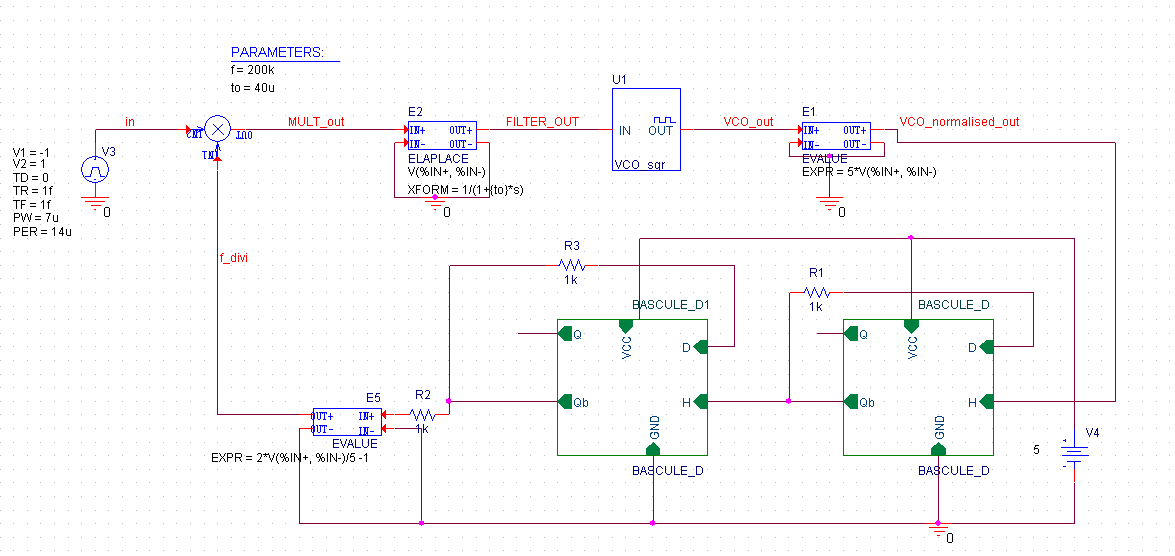
\includegraphics[width=\linewidth]{multi_sch.png}

\subsection{Résultats}

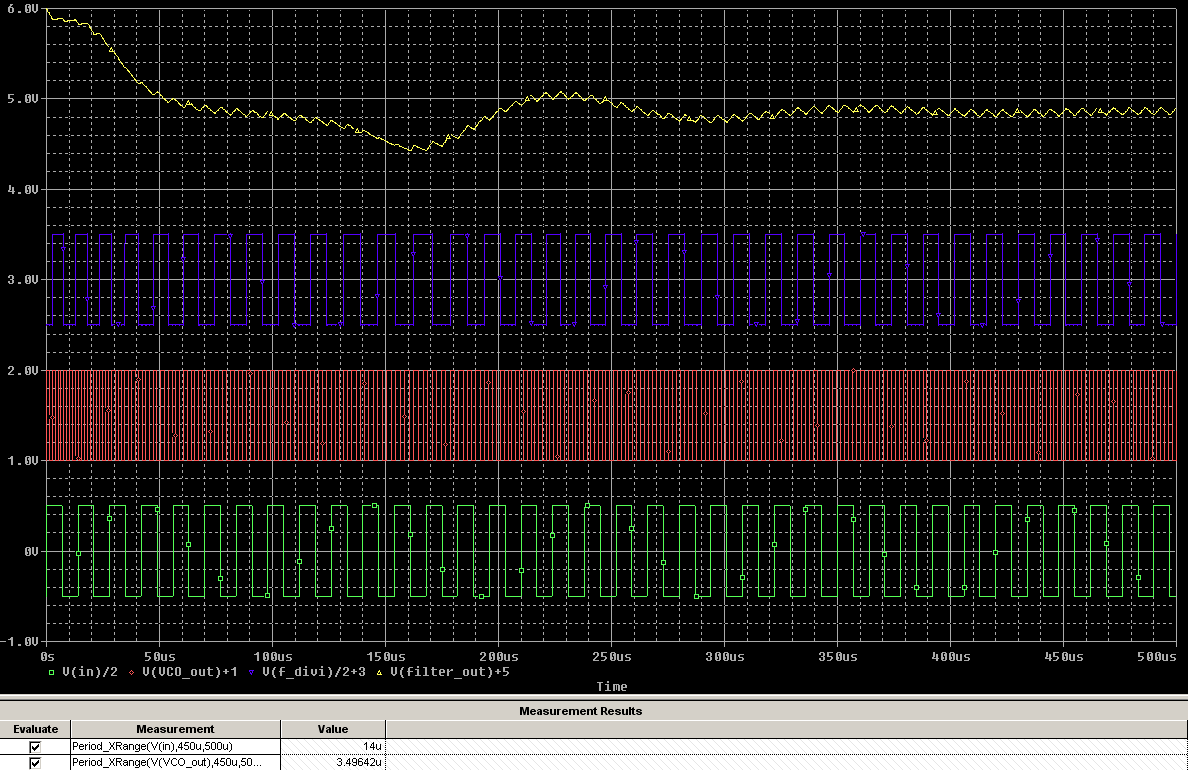
\includegraphics[width=\linewidth]{multi_sim.png}


\end{document}
